\documentclass[a4paper,12pt,openright,titlepage,oneside]{book}

%\usepackage[english,brazil]{babel} 
%Define regra de gramática para separar síbalas {babel}
%e altera os títulos (como chapters, sections, references) para português
\usepackage[brazil]{babel}

% Define uso de caracteres acentuados no PDF gerado
% e permite copiar corretamente o texto do PDF.
\usepackage[T1]{fontenc}
\usepackage[utf8]{inputenc}

% Adição do pacote do template da UnB
\usepackage{template-FT-UnB/ft2unb}

\DeclareGraphicsExtensions{.jpg,.pdf,.mps,.png,.gif, .eps}
\graphicspath{imagens} %define diretório de imagens

%Arquivo com lista com hifenização correta de algumas palavras.
%Defina novas palavras no arquivo a medida que verificar que a hifenização automática
%etá errada para tais palavras.
%----------------DEFINE FORMA CORRETA DE HIFENIZAÇÃO PARA ALGUMAS PALAVRAS ----------------
\hyphenation{cons-tru-a}
\hyphenation{e-xem-plo}
\hyphenation{e-xem-plar}
\hyphenation{e-le-men-to}
\hyphenation{e-le-men-tar}
\hyphenation{ma-nu-al}
\hyphenation{res-pos-ta}
\hyphenation{ca-rac-te-ris-ti-ca}
\hyphenation{ca-rac-te-ris-ti-cas}
\hyphenation{ca-rac-te-ris-ti-co}
\hyphenation{ca-rac-te-ris-ti-cos}
\hyphenation{cor-res-pon-den-ci-as}
\hyphenation{cons-tru-am}
\hyphenation{re-a-li-za-da}
\hyphenation{re-a-li-za-do}
\hyphenation{re-a-li-za-das}
\hyphenation{re-a-li-za-dos}
\hyphenation{i-ne-xis-ten-cia}
\hyphenation{i-ne-xis-te}
\hyphenation{e-xis-te}
\hyphenation{di-fe-ren-te}
\hyphenation{di-fe-ren-tes}
\hyphenation{dei-xan-do}
\hyphenation{ins-ta-la-do} 
\hyphenation{ins-ta-la-dos} 
\hyphenation{ins-ta-la-da}
\hyphenation{ins-ta-la-das}
\hyphenation{re-gis-tra-do}
\hyphenation{re-gis-tra-dos}
\hyphenation{re-gis-tra-da}
\hyphenation{re-gis-tra-das}
\hyphenation{des-cre-ve}
\hyphenation{res-pei-to}
\hyphenation{re-a-li-za}
\hyphenation{re-a-li-zar}
\hyphenation{a-tu-a-li-zar}
\hyphenation{a-tu-a-li-zan-do}
\hyphenation{a-tu-a-li-za-do}
\hyphenation{a-tu-a-li-za-da}
\hyphenation{fun-ci-o-na-li-da-de}
\hyphenation{pos-si-bi-li-da-de}
\hyphenation{dis-po-si-ti-vo}
\hyphenation{dis-po-si-ti-vos}
\hyphenation{e-xis-te}
\hyphenation{e-xis-tir}
\hyphenation{des-co-ber-ta}
\hyphenation{des-co-ber-to}
\hyphenation{de-sig-nar}
\hyphenation{de-sig-na-do}
\hyphenation{o-pe-ra-ci-o-nais} 
\hyphenation{o-pe-ra-ci-o-nal}
\hyphenation{con-si-de-ra-do}
\hyphenation{con-si-de-ra-dos}
\hyphenation{ou-tro}
\hyphenation{ou-tra}
\hyphenation{ou-tros}
\hyphenation{ou-tras}
\hyphenation{e-xis-ten-te}
\hyphenation{e-xis-ten-tes}
\hyphenation{LuaOnTV}
\hyphenation{De-fi-ni-tion}
%------------------------------------------------------------------------------------------ 

% ALTERE OS VALORES DENTRO DAS CHAVES DOS COMANDOS NESTA SEÇÃO PARA INCLUIR OS SEUS DADOS E DADOS DA SUA
% DISSERTAÇÃO DE MESTRADO OU TESE DE DOUTORADO
% -----------------------------------------------------------------------------------------------------

%\onehalfspacing
\title{DESEMPENHO DAS FORMAS DE ONDA CANDIDATAS AO 5G SOB EFEITO DE NÃO LINEARIDADES}
\author{SEU NOME COMPLETO}
\date{2011-03-16} %data da defesa

\grau{Mestre} %Mestre ou Doutor
\area{Engenharia Elétrica} %Nome do curso
\siglaarea{ENE} %Sigla do departamento
\tipodemonografia{Dissertação} %Dissertação ou Tese
\programa{Mestrado} %Mestrado ou Doutorado
\autorendereco{SEU ENDEREÇO COMPLETO AQUI.} %Endereço do autor da dissertação/tese
\totalpgs{147} %total de páginas atualmente na sua dissertação
\dia{18} %dia da defesa
\mes{Dezembro} %mês da defesa
\ano{2017} %ano da defesa
\numpublicacao{xxx/AAAA} %número da publicação (após a defesa, tal número deve ser obtido na secretaria)

%PPGENE.DM  = Programa de Pós Graduação em ENgenharia Elétrica.Dissertação de Mestrado
%PPGENE.TD  = Programa de Pós Graduação em ENgenharia Elétrica.Tese de Doutorado
\siglapublicacao{PPGENE.DM}

\titulolinhai{DESEMPENHO DAS FORMAS DE ONDA CANDIDATAS AO 5G}
\titulolinhaii{SOB EFEITO DE NÃO LINEARIDADES}
\titulolinhaiii{}
\titulolinhaiv{}

\autori{VANESSA DE OLIVEIRA VASCONCELLOS}
%Caso seu nome não caiba em uma única linha, divida ele nos comandos abaixo
%\autorii{} 
%\autoriii{}

\membrodabancai{Prof. Dr. ANDRE NOLL BARRETO, ENE/UnB}
\membrodabancaifuncao{Orientador}
\membrodabancaii{Prof. Dr. Judson Braga, ENE/UnB}
\membrodabancaiifuncao{Examinador interno}
\membrodabancaiii{Prof. Dr. Ugo Dias, ENE/UnB}
\membrodabancaiiifuncao{Examinador interno}
\membrodabancaiv{Prof. Luciano Leonel , INATEL/MG}
\membrodabancaivfuncao{Examinador externo}
\membrodabancav{}
\membrodabancavfuncao{}
% -----------------------------------------------------------------------------------------------------

%line-numbers, inputencoding=utf8/latin1
%Define o estilo para listagens de código fonte
\lstset{
  numbers=left, %numeração de linhas à esquerda
  stepnumber=1,
  firstnumber=1,
  numberstyle=\tiny,
  extendedchars=true,
  frame=none,
  basicstyle=\footnotesize,
  stringstyle=\ttfamily,
  showstringspaces=false,
  %language=Java, %deve ser definida na inclusão de cada trecho de código, pois podem existir linguagens diferentes em exemplos diferentes
  breaklines=true,
  breakautoindent=true,
  %estilos de comentário de uma e várias linhas
  morecomment=[l]{--}, morecomment=[s]{/*}{*/}, morecomment=[s]{<!--}{-->}, morecomment=[s]{--[[}{--]]}
}

% Adição de metadados no PDF (propriedades do documento PDF)
\makeatletter
	 \hypersetup{
		 pdftoolbar=true,        % show Acrobat’s toolbar?
		 pdfmenubar=true,        % show Acrobat’s menu?
		 pdffitwindow=false,     % window fit to page when opened
		 pdfstartview={FitH},    % fits the width of the page to the window	 
		 pdftitle={\@title},
		 pdfauthor={\@author},
		 pdfsubject={\tipodemonografianome \ de\ \programastr \ em\ \areastr},   % subject of the document
		 pdfcreationdate={\pdfdate}
	 }
\makeatother


\makeindex
\makenomenclature %Necessário para gerar lista de siglas


\begin{document}

	\pdfbookmark[0]{Agradecimentos}{agradecimentos}
	%* indica para nao adicionar numeracao ao titulo
\chapter*{Agradecimentos}

Inclua seus agradecimentos aqui.
	Inclua o resumo aqui.
	
	\pdfbookmark[0]{Sumário}{sumario}
	\sumario
	
	\pdfbookmark[0]{Lista de Figuras}{listafiguras}
	\listadefiguras
	
	\pdfbookmark[0]{Lista de Tabelas}{listatabelas}
	\listadetabelas
	
	\pdfbookmark[0]{Lista de Códigos Fonte}{listacodigosfonte}
	\listadecodigosfonte
	
	\renewcommand{\nomname}{LISTA DE TERMOS E SIGLAS} %Define um caption à lista de siglas
	%Inclui a lista de siglas 
	\pdfbookmark[0]{Lista de Termos e Siglas}{nomenclatura}
	\printnomenclature[2.5cm] 
	
	\mainmatter %Inicia a numeracao normal cardinal
	\setcounter{page}{1} \pagenumbering{arabic} \pagestyle{plain}
	
	\chapter{Introdução} \label{introducao}

Este trabalho Lorem ipsum dolor sit amet, consectetuer adipiscing elit. Ut purus elit, vestibulum ut, placerat ac, adipiscing vitae, felis. Curabitur dictum gravida mauris. Nam arcu libero, nonummy eget, consectetuer id, vulputate a, magna. Donec vehicula augue eu neque. Pellentesque habitant morbi tristique senectus et netus et malesuada fames ac turpis egestas. Mauris ut leo. Cras viverra metus rhoncus sem. Nulla et lectus vestibulum urna fringilla ultrices. Phasellus eu tellus sit amet tortor gravida placerat. Integer sapien est, iaculis in, pretium quis, viverra ac, nunc. Praesent eget sem vel leo ultrices bibendum. Aenean faucibus. Morbi dolor nulla, malesuada eu, pulvinar at, mollis ac, nulla. Curabitur auctor semper nulla. Donec varius orci eget risus. Duis nibh mi, congue eu, accumsan eleifend, sagittis quis, diam. Duis eget orci sit amet orci dignissim rutrum.

Nam dui ligula, fringilla a, euismod sodales, sollicitudin vel, wisi. Morbi auctor lorem non justo. Nam lacus libero, pretium at, lobortis vitae, ultricies et, tellus. Donec aliquet, tortor sed accumsan bibendum, erat ligula aliquet magna, vitae ornare odio metus a mi. Morbi ac orci et nisl hendrerit mollis. Suspendisse ut massa. Cras nec ante. Pellentesque a nulla. Cum sociis natoque penatibus et magnis dis parturient montes, nascetur ridiculus mus. Aliquam tincidunt urna. Nulla ullamcorper vestibulum turpis. Pellentesque cursus luctus mauris.

O trabalho está organizado como segue. O capítulo  \ref{capitulo1} apresenta detalhes sobre a arquitetura proposta. O capítulo \ref{capitulo2} apresenta os protocolos de comunicação utilizados. Por fim, o capítulo \ref{conclusao} apresenta as conclusões e trabalhos futuros propostos.
	\chapter{Arquitetura de comércio eletrônico para a TV Digital} \label{capitulo1}
%label cria um rótulo para o objeto, para permitir que ele seja referenciado com o comando \ref{nome-do-rotulo}


Neste capítulo é apresentada uma arquitetura para provimento de comércio eletrônico
para o Sistema Brasileiro de TV Digital (SBTVD) \nomenclature{SBTVD}{Sistema Brasileiro de TV Digital}. A mesma é uma arquitetura distribuída, baseada em componentes
reutilizáveis, os \textit{Web Services}, conhecida como Arquitetura Orientada a Serviços.

Segundo \cite{soares2007ginga}:

\begin{quote}
	Lorem ipsum dolor sit amet, consectetuer adipiscing elit. Ut purus elit, vesti- bulum ut, placerat ac, adipiscing vitae, felis. Curabitur dictum gravida mauris. Nam arcu libero, nonummy eget, consectetuer id, vulputate a, magna. 
\end{quote}

Desta forma, a arquitetura proposta foi definida, incluindo a implementação de um \textit{framework} de comunicação (baseado nos protocolos HTTP e SOAP) que é apresentado sucintamente neste capítulo, e em mais detalhes no Capítulo \ref{capitulo2}. Mais detalhes podem ser consultados em \cite{soares2007ginga}. Veja um exemplo na Listagem \ref{list:server}, que foi adaptada de \url{http://manoelcampos.com}.

Lorem ipsum dolor sit amet, consectetuer adipiscing elit. Ut purus elit, vestibulum ut, placerat ac, adipiscing vitae, felis. Curabitur dictum gravida mauris. Nam arcu libero, no- nummy eget, consectetuer id, vulputate a, magna. Donec vehicula augue eu neque. Pel- lentesque habitant morbi tristique senectus et netus et malesuada fames ac turpis egestas. Mauris ut leo. Cras viverra metus rhoncus sem. Nulla et lectus vestibulum urna fringilla ultrices. Phasellus eu tellus sit amet tortor gravida placerat. Integer sapien est, iaculis in, pretium quis, viverra ac, nunc. Praesent eget sem vel leo ultrices bibendum. Aenean fauci- bus. Morbi dolor nulla, malesuada eu, pulvinar at, mollis ac, nulla. Curabitur auctor semper nulla. Donec varius orci eget risus. Duis nibh mi, congue eu, accumsan eleifend, sagittis quis, diam. Duis eget orci sit amet orci dignissim rutrum.

Nulla malesuada porttitor diam. Donec felis erat, congue non, volutpat at, tincidunt tristi- que, libero. Vivamus viverra fermentum felis. Donec nonummy pellentesque ante. Phasellus adipiscing semper elit. Proin fermentum massa ac quam. Sed diam turpis, molestie vitae, placerat a, molestie nec, leo. Maecenas lacinia. Nam ipsum ligula, eleifend at, accumsan nec, suscipit a, ipsum. Morbi blandit ligula feugiat magna. Nunc eleifend consequat lorem. Sed lacinia nulla vitae enim. Pellentesque tincidunt purus vel magna. Integer non enim. Praesent euismod nunc eu purus. Donec bibendum quam in tellus. Nullam cursus pulvinar lectus. Donec et mi. Nam vulputate metus eu enim. Vestibulum pellentesque felis eu massa. 

\lstset{caption=Exemplo de aplicação servidora, label=list:server}
\begin{lstlisting}[language=C]
int main()
{ 
    FILE *fp;     int len;     
    static const int SIZE = 1024;
    struct sockaddr_in me, target;
    int sock=socket(AF_INET,SOCK_DGRAM,0);
    char arquivo[SIZE];
    me.sin_family=AF_INET;
    me.sin_addr.s_addr=htonl(INADDR_ANY); // endereco IP local 
    me.sin_port=htons(0); // porta local (0=auto assign)
    bind(sock,(struct sockaddr *)&me,sizeof(me));
    target.sin_family=AF_INET;
    target.sin_addr.s_addr=inet_addr("192.168.68.217"); // host local 
    target.sin_port=htons(8450); // porta de destino 

    if ((fp = fopen("video1.mp4","rb")) == NULL){
        printf("Arquivo nao pode ser aberto.\n"); return -1;
    }

    while(!feof(fp)) {
        len = fread(arquivo, 1, sizeof(arquivo), fp);
        sendto(sock,arquivo,sizeof(arquivo),0,(struct sockaddr *)&target,sizeof(target));
    }
    sendto(sock,"FIM",sizeof("FIM"),0,(struct sockaddr *)&target,sizeof(target));
    close(sock);
    return 0;
}
\end{lstlisting}

	\chapter{\textit{Orthogonal Filter Bank Mutlicarrier} - OFDM} \label{capitulo2}

O OFDM é uma forma de onda bastante conhecida. Aqui, mais do que se apresentar a arquitetura utilizada para construção e detecção deste tipo de sinal, deseja-se mostrar como este tipo de símbolo continuará a ser utilizado em sistemas 5G e quais adaptações serão necessárias se houver alguma. Na próxima seção, introduz-se o leitor ao sistema. 

\section{Arquitetura OFDM}\label{pulso} 

\par O OFDM é uma tecnologia descoberta  há algumas décadas \ref{tcc1}, mas que somente entrou em uso recentemente, quando a tecnologia disponível em termos de software e circuitos eletrônicos, aliada às necessidades do mercado, possibilitaram sua aplicação prática.
\par Esta forma de onda é um caso especial do FDM (Frequency Division Multiplexing), uma técnica que data dos anos 1910 \cite{tcc1}, em que uma largura de banda larga é dividia entre vários usuários, sendo cada um deles alocados a uma faixa de frequências distinta. 
\par À época da telegrafia, fazia-se uso do TDM (“Time Divsion Multiplexing”), em que usuários eram alocados em slots de tempo de forma alternada. O sistema possuía algumas limitações, o que incentivava a busca por novas formas de alocar recursos do canal. Foi nesse contexto que surgiu a hipótese  da transmissão FDM \cite{tcc1}. 
\par Nomes como Alexander Graham Bell, Elisha Gray e Thomas Edison trabalharam no desenvolvimento desta tecnologia, tendo o primeiro se dedicado a aplicações desta na telefonia e não apenas na comunicação telegráfica.
\par O FDM tornou-se a base da telefonia analógica em 1918, sendo substituído por um sistema misto (TDM/FDM) nos anos 1970 e posteriormente por outro, unicamente TDM \cite{tcc1}.
\par Com o crescimento do número de usuários, o TDM tornou-se obsoleto e o FDM voltou a ser aplicado, mas em uma versão aprimorada. As informações passaram a ser transmitidas por canais mais estreitos, o que aumentou a imunidade destes a canais de multipercursos. Além disso, a equalização do sinal recebido tornou-se mais simples. 
\par Como qualquer sistema, o FDM também possui desvantagens. Para que não haja interferência entre canais adjacentes, é necessária a alocação de uma banda de guarda entre eles, um desperdício de recurso espectral. Outro problema é sua alta complexidade, já que são necessários moduladores ajustados à frequência de cada canal. 
\par Buscando solucionar estes inconvenientes, surge o conceito do OFDM, um sistema FDM com canais sobrepostos, mas não interferentes. Uma escolha simples que possibilita essas características são as portadoras regidas por funções senoidais harmônicas, que são ortogonais dentro do período fundamental. 		
Em um sistema OFDM, as $M$ subportadoras são representadas por $Re\{e^{j(2 \pi f_{m})}\}_{m = 0}^{M-1}$, $f_{m} = \frac{m+1}{T}$, em que $T$ é a duração do símbolo OFDM transmitido. Um bloco de sinal OFDM pode ser definido, então, como a soma de várias ondas senoidais de frequências distintas, pensando em cada uma como um subcanal. Na ausência de distorções, estes subcanais não se interferem, já que os pontos de máximo de uma subportadora coincidem com o de zero das outras. A Figura \ref{subportadorasOFDM}mostra este efeito da ortogonalidade em um sistema OFDM.

\begin{figure}[h!]
\centering
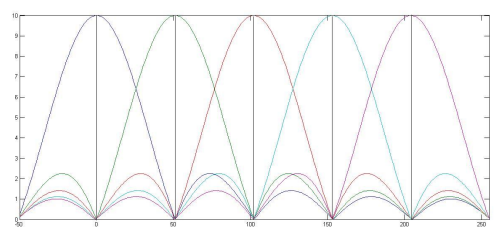
\includegraphics[width=3.5in]{fig_OFDM_freq.png} %Trocar para subortadoras OFDM
\caption{Subportadoras OFDM}
\label{subportadorasOFDM}
\end{figure}

\par A representação das subportadoras OFDM remete a uma função conhecida: a transformada inversa de Fourier – dada pela IDFT (Inverse Descrete Fourier Transform) no domínio discreto dos símbolos transmitidos, como será visto na seção \ref{trans_OFDM}  

\subsection{TRANSMISSOR OFDM}\label{trans_OFDM}
\par O transmissor OFDM é caracterizado da seguinte forma: primeiro, uma sequência de bits é mapeada em uma sequência de símbolos $X[k]$, M-PSK ou M-QAM. Esta sequência de símbolos em série é convertida em N fluxos de símbolos paralelos e cada um deles é transmitido por uma subportadora diferente $f_{m} =  \frac{m+1}{T}$, como mostra a Figura \ref{trans1OFDM} \cite{tcc9}.

\begin{figure}[h!]
\centering
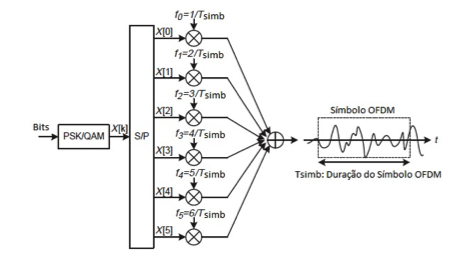
\includegraphics[width=3.5in]{trans_OFDM.png} %Trocar para subortadoras OFDM
\caption{Transmissior OFDM \cite{tcc9}}
\label{trans1OFDM}
\end{figure}

\par O símbolo OFDM transmitido pode ser escrito, no tempo discreto, como \cite{tcc9}

\begin{equation}\label{IDFTsimb}
x_{l}[n] = \sum_{k=0}^{M-1}X_{l}[k]e^{(j\frac{2\pi m n}{M})}, m=0,1,…,M-1,
\end{equation}

em que a equação \ref{IDFTsimb} representa a IDFT dos símbolos $X_{l}[k]_{k=0}^{M-1}$, que pode ser eficientemente computada por meio de do algoritmo de IFFT (Inverse Fourier Transform) \cite{tcc9}. Nesta equação, o subíndice l representa o l-ésimo símbolo transmitido na k-ésima suportadora.  O transmissor OFDM com o bloco IFFT é mostrado na Figura \ref{transIFFT}.

\begin{figure}[h!]
\centering
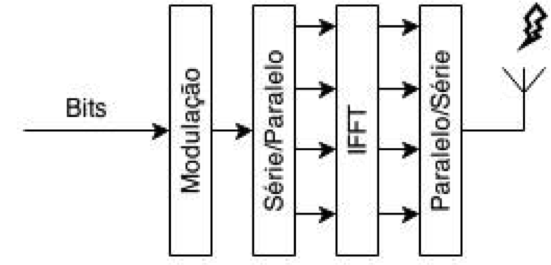
\includegraphics[width=3.5in]{transOFDMIFFT.png} %Trocar para sistema FDM
\caption{Transmissor OFDM com IFFT}
\label{transIFFT}
\end{figure}

\par O sistema OFDM da maneira que foi descrito acima só funcionaria na ausência de qualquer perturbação externa. Um efeito que traria grandes perturbações, seria a presença de um canal de multipercursos na transmissão, como será visto na Subseção \ref{multipercurso}. 

\subsection{Efeitos do Canal de Multipercursos}\label{multipercurso}

Seja o i-ésimo símbolo OFDM dado por \cite{tcc9}

\begin{equation}
x_{l}(t) = \sum_{m=0}^{M-1}X_{l}[m]e^{j 2 \pi f_{m}(t-lT)}
\end{equation}
	
\par Para um canal com resposta ao impulso $c_{l}(t)$, o sinal recebido será \cite{tcc9}:

\begin{equation}\label{eq3}
y_{l} (t)= x_{l}(t)\ast c_{l}(t)+ z_{l}(t)= \int_{0}^{\infty} c_{l}(t)x_{l}(t-\tau)dt+ z_{l}(t)
\end{equation}

em que, $z(t)$ representa ruído AWGN (Additve Gaussian White Noise – Ruído Branco Gaussiano Aditivo). No domínio discreto, a equação \ref{eq3} pode ser escrita como \cite{tcc9}:

\begin{equation} \label{eq4}
y_{l} = x_{l}[n] \ast c_{l}[n] + z_{l}[n] = \sum_{m=0}^{\infty}h_{l}[k]x_{l}[n-k]+z_{l}[n]
\end{equation}
	
\par Agora, se supõe que todo o segundo símbolo OFDM é enviado imediatamente após a última amostra do primeiro símbolo OFDM. Em acordo com a equação \ref{eq4}, o primeiro símbolo OFDM será prolongado no tempo, interferindo, portanto, nas amostras iniciais do segundo, como é mostrado pelo destaque em vermelho na Figura \ref{multichan}
	
\begin{figure}[h!]
\centering
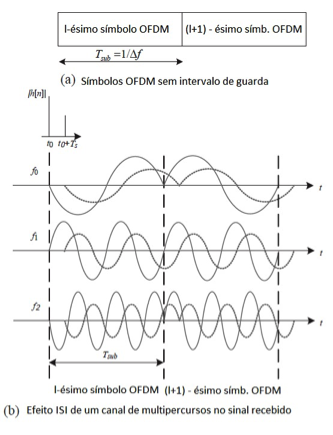
\includegraphics[width=3.5in]{ISIOFDM.png} %Trocar para sistema FDM
\caption{Interferência Intersimbólica \cite{tcc9}}
\label{multichan}
\end{figure}

\par É bastante intuitivo acrescentar um intervalo de guarda entre os símbolos OFDM. Este intervalo deve ser tal que sua duração supere o máximo atraso gerado pelo canal.  
\par Em vez de esperar um intervalo de tempo para o envio do próximo símbolo (zero-padding), é mais interessante construir o intervalo de guarda como mostra a Figura \ref{cp}

\begin{figure}[h!]
\centering
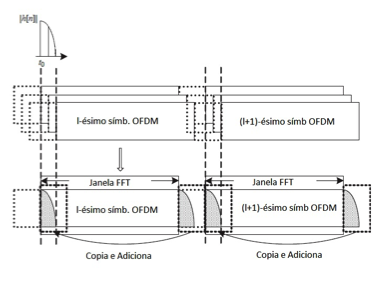
\includegraphics[width=3.5in]{cp.png} %Trocar para CP
\caption{Prefixo Cíclico  \cite{tcc9}}
\label{cp}
\end{figure}
		
\par A Figura \ref{cp} é a ilustração do processo conhecido por “inserção de prefixo cíclico”. A grande vantagem deste procedimento é a possibilidade de recuperação do sinal recebido por meio de da transformada de Fourier, como mostra o anexo I desta dissertãção. Na próxima seção apresenta-se o receptor OFDM. 

\subsection{Receptor OFDM}

\par No receptor, de forma geral, são desfeitos os passos do transmissor, como mostra a Figura \ref{rec_OFDM}.	

\begin{figure}[h!]
\centering
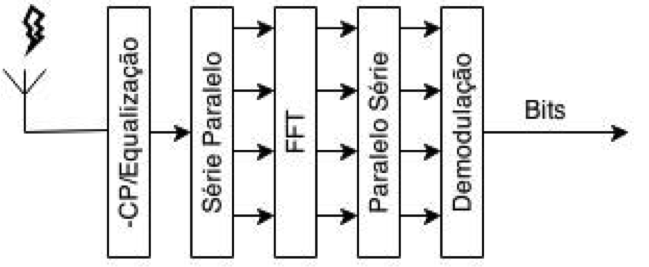
\includegraphics[width=3.5in]{recOFDM.png} %Trocar receptor OFDM
\caption{Receptor OFDM  \cite{tcc9}}
\label{rec_OFDM}
\end{figure}	

\par Primeiramente, o prefixo cíclico é eliminado. Após sua retirada, a equalização de um tap é realizada \ref{equalizationOFDM}:

\begin{equation}\label{equalizationOFDM}
x_{l}[n]=IFFT\{FFT\{(Y_{l}[m])/(H_{l}[m])\}\}
\end{equation}

\par Os símbolos $x_{l}[n]$ em série são convertidos em símbolos em paralelo e posteriormente demodulados, retornando às suas bandas-base por meio da FFT. O procedimento seguinte é a conversão paralelo-série, seguido pela demodulação. Finalmente, são obtidas estimativas dos bits enviados pelo transmissor. 

\begin{figure}[h!]
\centering
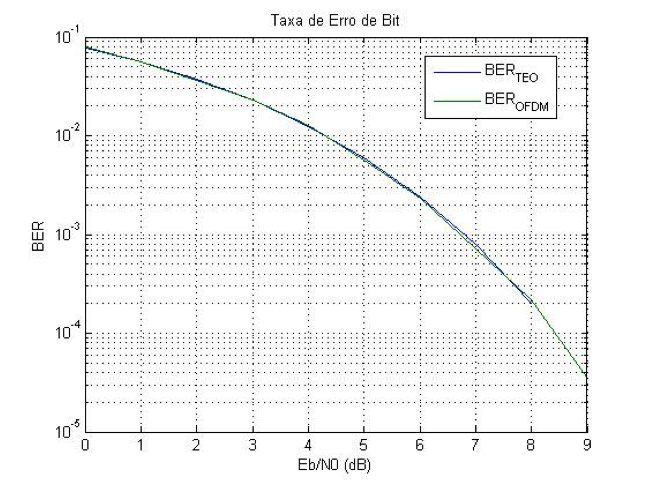
\includegraphics[width=3.5in]{BER_TEO.png} 
\caption{BER QPSK}
\label{taxa_erros}
\end{figure}

\par A taxa de erros desta estimativa na recepção é mostrada na Figura \ref{taxa_erros}. Esta figura foi obtida por meio de de simulação no software MATLAB© e os parâmetros utilizados são mostrados na tabela \ref{tab_sim}. 

\begin{center} \label{tab_sim}
\begin{tabular}{ c c}
Número de Subportadoras & 300  \\ 
Prefixo Cíclico & 32 \\  
Número de Símbolos & 50 \\
\end{tabular}
\end{center}

\par Percebe-se a partir da Figura 2.8, que o OFDM tem um desempenho próximo ao esperado para um sistema de portadoras únicas ($BER_{TEO}$). É válido ressaltar a queda de desempenho do sistema OFDM é causada pelo prefixo cíclico, que leva a um certo desperdício de energia.  
\par Até aqui, pode-se observar a existência de algumas vantagens no uso do OFDM:
\begin{itemize}	
    \item implementação Digital por meio da FFT/IFFT;
	\item eficiência espectral em comparação aos sistemas FDM comuns.
	\item taxa de erro de bits aceitável;
	\item equalização cuja complexidade independe do canal.
\end{itemize}   
\par Devido a estas vantagens, o sistema OFDM passou a ser aplicado em diferentes sistemas de comunicação. Alguns deles serão descritos na próxima seção, que abrange, também, as expectativas 5G para o OFDM.

\section{Aplicações OFDM - 4G x 5G}

\subsection{F-OFDM}
\subsection{ZT-DS-OFDM}



\section{Desempenho sob o efeito de não linearidades }
 



 
	%Usar \chapter*{Título do Capítulo} faz com que o capítulo não seja numerado
\chapter{Conclusão} \label{conclusao}

Insira sua conclusão aqui. 
		
	\bibliographystyle{abnt-num} % estilo bibliográfico ABNT numérico
	\bibliographystyle{abnt-alf} % estilo bibliográfico ABNT alfabético
	\bibliographystyle{sbc}  % estilo bibliográfico da Sociedade Brasileira de Computação (SBC)
	
   \renewcommand{\bibname}{REFERÊNCIAS BIBLIOGRÁFICAS} %Define o Caption da seção de bibliografia
	\addcontentsline{toc}{chapter}{REFERÊNCIAS BIBLIOGRÁFICAS}
    
    \bibliography{referencias}

    


	Chapter*{Modelos de Amplificadores Não Lineares} \label{apendix II}

\par Amplificadores de potência (PA) são dispositivos essenciais nas comunicações RF. Geralmente, apresentam um comportamento linear somente para um intervalo limitado de entrada: quanto maior for a amplitude deste sinal, mais próximo da saturação estará o PA, o que pode levar a distorção do sinal amplificado e limitar a eficiência energética. 
\par Fica claro que, ao projetar um sistema com amplificação, existirá uma troca entre linearidade e eficiência \cite{Bhat}. Para ilustrar essas afirmações, dois modelos de amplificadores são apresentados: um que desconsidera os efeitos de memória e outro que os leva em conta. 
 
\begin{enumerate} 
\item {Amplificadores Sem Memória} 

Amplificadores sem memória são dispositivos não lineares para os quais a saída não depende das amostras anteriores da entrada. Isso é o caso, geralmente, de amplificadores de estado sólido (SSA), os quais seguem o modelo Rapp \cite{Rapp}. Matematicamente, são representados por: 

\begin{equation} \label{x}
x(t) = A(t)e^{j\Psi(t)}
\end{equation}

em que $x$(t) é o sinal de entrada do amplificador de potência, com amplitude $A(t)$ e fase $\Psi(t)$. 

\par A saída vai ser dada como se segue \cite{Uilian2}:
\begin{equation} \label{y}
y(t) = G[A(t)] e^{\{j\Psi(t)+ \Phi[A(t)]\}} 
\end{equation}
na qual $G[A(t)]$ é o fator de conversão AM$/$AM e $\Phi[A(t)]$ o fator AM$/$PM do PA. Para o modelo Rapp, o comportamento da fase, contabilizado por \textit{$\Psi$(t)}, pode ser descartado \cite{Uilian2}. A parte importante é $G[A(t)]$: 

\begin{equation} 
\label{GA}
G(A)= \frac{\nu A}{\left[1+ \left(\frac{A}{A_0} \right)^{2p} \right]^{1/2p}} 
\end{equation}
em que $\nu$ é o ganho de pequenos sinais, $A_0$ é a amplitude de saturação e $p$ é o fator de \textit{smoothness} ("suavização"). 

Para os resultados encontrados nos capítulos 4 a 5, considerou-se $A_0 =1$ and $p=3$. A função de transferência (\ref{GA}) para estes parâmetros é exibida na Figura \ref{FTrans}: 

\begin{figure}[h!]
\centering
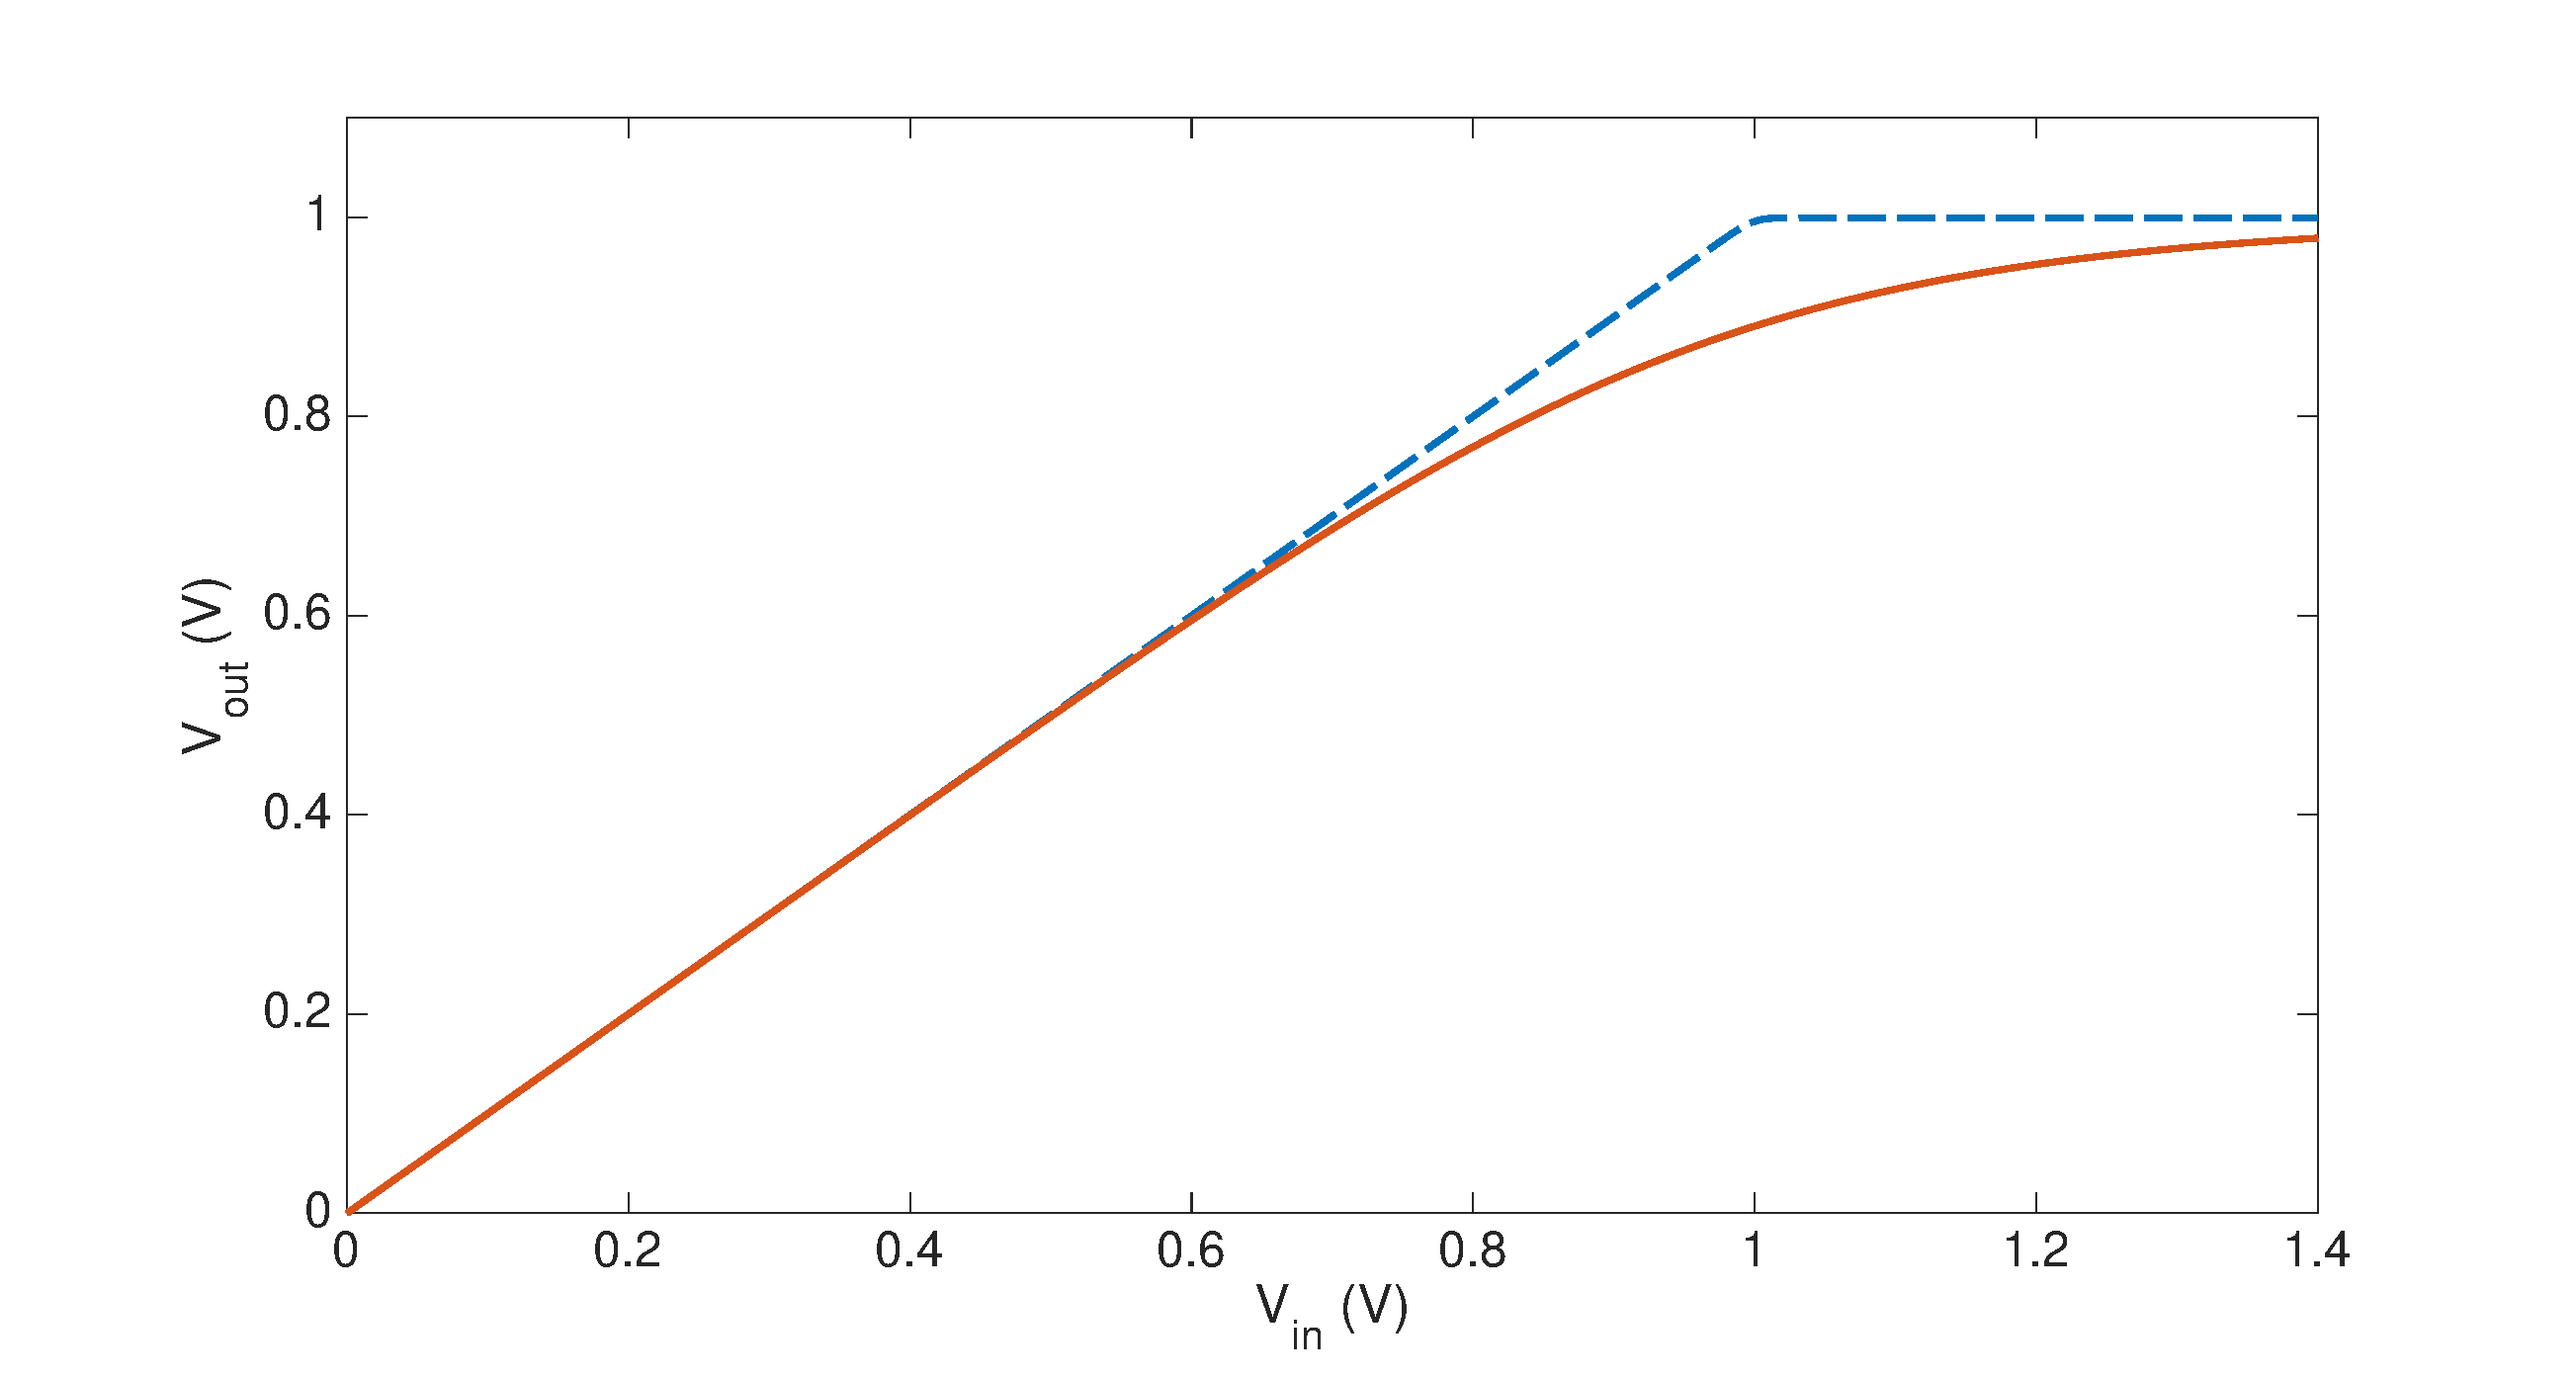
\includegraphics[width=3.5in]{HPA}
\caption{Transfer function of the non-linear amplifier.}
\label{FTrans}
\end{figure}

\item{Ampificadores de Potência com Memória} 
Nessa seção, efeitos de memória, que são comuns em amplificadores TWT são estudados. Para modela-los, será utilizada uma ferramenta matemática chamada Série de Volterra. Ems ua forma geral, esta é representada por: \cite{Morgan2006}: 

\begin{equation} 
\label{poly}
y(n)= \sum_{k=1}^{M-1}y_{k}(n),   
\end{equation}

em que 

\begin{equation} 
\label{kernel}
y_{k}(n)= \sum_{m_{1}=0}^{M-1}\dots\sum_{m_{k}=0}^{M-1}h_{k}(m_{1},\dots,m_{k})\prod_{l=1}^{k}y_{k}(n)  
\end{equation}

A equação (\ref{kernel}) é uma convolução multi-dimensional. O índice no tempo $m_{k}$ representa qual amostra do passado impacta no sinal do presente e $M$ é o comprimento da memória. Por simplicidade, no presente trabalho não se utilizou a série completa. Em \cite{Ding2004}, foi visto que é possível reduzir a equação do PA utilizando somente o polinômio de ordem ímpar: 

\begin{equation} 
\label{oddpoly}
y(n)= \sum_{k_{1}=0}^{K}\sum_{q=0}^{Q}c_{kq}z(n-q)|z(n-q)|^{k-1}
\end{equation}

Os coeficientes propostos foram extraídos, também de  \cite{Ding2004} e modelam um amplificador classe AB. Na análise, o comprimento de memória ($M$) é considerado $2$ e o grau do polinômio ($Q$) é $5$.  

\end{enumerate}

\end{document}

